\documentclass[pdflatex,compress]{beamer}

%\usetheme[dark,framenumber,totalframenumber]{ElektroITK}
\usetheme[darktitle,framenumber,totalframenumber]{ElektroITK}

\usepackage{lipsum}

\title{PENGOLAHAN SINYAL DIGITAL}
\subtitle{Sinyal dan Sistem Waktu Diskrit}

\author{Tim Dosen Pengampu}

\begin{document}

\maketitle

\section{Pendahuluan}

\begin{frame}
	\frametitle{Pengantar}
	\begin{itemize}
		\item Sinyal dan sistem waktu diskrit memiliki beberapa kesamaan dengan sinyal dan sistem waktu kontinyu.
		\item Beberapa kasus yang ada di sinyal dan sistem waktu kontinyu memiliki beberapa kesamaan dengan sinyal dan sistem waktu diskrit, yang mana akan kita pelajari sepanjang perkuliahan ini.
		\item Namun, juga ada beberapa perbedaan antara sinyal dan sistem waktu diskrit dengan sinyal dan sistem waktu kontnyu.
		\item Perbedaan-perbedaan ini sangat penting dan perlu kita pahami dengan baik.
	\end{itemize}
\end{frame}

\begin{frame}
	\frametitle{Pengantar}
	\begin{itemize}
		\item Dalam domain waktu diskrit, sinyal yang diproses adalah berupa sequences $\rightarrow$ sinyal merupakan fungsi dari variabel bilangan bulat/ \textbf{integer} ($ n $).
		\item Pada slide selanjutnya, diilustrasikan contoh dari \textbf{general sequence} $ x(n) $, sebuah fungsi energi dari variabel $ n $, dan nilai dari sequence-nya dinyatakan dalam bar dengan tinggi sesuai dengan nilai sequence-nya.
		\item Perlu diperhatikan bahwa variabel $ n $ \textbf{harus berupa integer}. Jika bukan integer, maka $ x(n) $ tidak terdefinisikan.
		\item Apapun argument dalam fungsi tersebut harus bernilai \textbf{integer}.
	\end{itemize}
\end{frame}

\begin{frame}
	\frametitle{General Sequence}
	% TODO: \usepackage{graphicx} required
	\begin{center}
		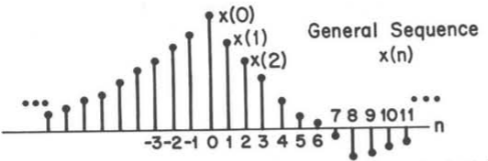
\includegraphics[width=\linewidth]{img/img001}
	\end{center}
\end{frame}

\begin{frame}
	\frametitle{Basic Sequence}
	\begin{itemize}
		\item Sama seperti di domain waktu kontinyu, pada domain waktu diskrit juga memiliki \textbf{basic sequence}.
		\item Basic sequence yang pertama adalah \textbf{unit sample} yang diilustrasikan pada slide selanjutnya.
	\end{itemize}
\end{frame}

\begin{frame}
	\frametitle{Unit Sample}
	% TODO: \usepackage{graphicx} required
	\begin{center}
		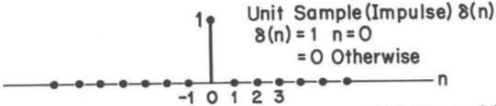
\includegraphics[width=\linewidth]{img/img002}
	\end{center}
\end{frame}

\begin{frame}
	\frametitle{Unit Step}
	% TODO: \usepackage{graphicx} required
	\begin{center}
		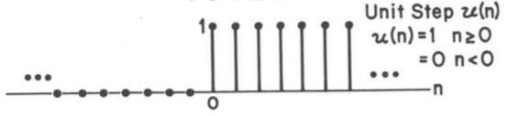
\includegraphics[width=\linewidth]{img/img003}
	\end{center}
\end{frame}

\end{document}
